\documentclass[a4paper, 12pt, openright, oneside, german, french, english, brazil, article]{abntex2}
\usepackage[brazil]{babel}
\usepackage{graphicx}
\usepackage[utf8]{inputenc}
\usepackage{graphicx}
\usepackage{wrapfig}
\usepackage{lscape}
\usepackage{rotating}
\usepackage{epstopdf}
\usepackage[alf]{abntex2cite}
\usepackage[a4paper, left=3cm, right=2cm, top=3cm, bottom=2cm]{geometry}
\usepackage{indentfirst}
\usepackage{longtable}
\pagestyle{plain}

\titulo{\textbf{A Construção Social de Prestígio e Valor no Mercado da Música Erudita}}
\autor{Neylson J. B. F. Crepalde}
\data{Agosto, 2016}
\instituicao{UNIVERSIDADE FEDERAL DE MINAS GERAIS
	\par
	Faculdade de Filososia e Ciências Humanas}
\local{Belo Horizonte}
\orientador{Dr. Silvio Salej Higgins (PPGS -- UFMG)}

\coorientador{Dr. Emmanuel Lazega (Sciences Po, CSO -- Paris)}
\preambulo{Projeto de Pesquisa apresentado ao Programa de Pós-Graduação em Sociologia da UFMG como requisito para ingresso no Programa Doutorado Sanduíche no Exterior (PDSE).}
%\tipotrabalho{Tese (doutorado)}


\begin{document}
\pretextual
\imprimirfolhaderosto

\textual
\section{Introdução}

Este trabalho visa debruçar-se sobre o mercado da música de concerto na região Sudeste do Brasil. A investigação é norteada por duas principais perguntas: 1) Entendendo que o mercado das orquestras não opera como um mercado comum, como se dá seu funcionamento; quem são os atores envolvidos e quais são as ações que cada um desenvolve no sistema? 2)Quais são as condições e fatores sociais de produção de padrões de qualidade da música de concerto, ou seja, como é produzido e mantido o \textit{standard} de qualidade com o qual todos estão comprometidos?

Para desenvolvermos nosso estudo faz-se necessário transcender os limites com os quais a teoria econômica se deparou ao abordar produtos culturais. Ora, em todo o seu decurso, a teoria econômica tem ancorado seus principais achados em dois pressupostos. O primeiro remonta à ideia do \textit{homo economicus}, ou seja, o ator racional que toma decisões visando potencializar ganhos e diminuir perdas. Para isso, ele tem acesso à completude das informações de que precisa e é capaz de processá-las inteiramente. Esse pressuposto dá à economia a capacidade de elaborar modelos elegantes para explicar escolhas e preferências mas não consegue incorporar uma parte central da vida social, a saber, a cultura. A área da sociologia econômica desenvolveu-se, sobretudo, se debruçando sobre as lacunas deixadas por esse pressuposto buscando dar conta de como normas sociais, valores, sistemas de status e prestígio influenciam a ação econômica. Dito de outra forma, uma perspectiva sociológica possibilita enxergar fatores relacionais que ajudam a responder a perguntas clássicas da economia além de tornar o estudo mais próximo da realidade mesmo não tendo modelos tão elegantes e nem lógica tão consistente \cite{hirsch1987dirty}. A sociologia econômica está preocupada com elementos contextuais das trocas econômicas, ou seja, analisar como as interações entre os atores fazem emergir um mercado e como essas interações regulam e controlam os mercados.





O segundo pressuposto consiste da caracterização geral dos produtos mercantis. As mercadorias são entendidas por meio de quatro critérios objetivos, a saber, suas propriedades físicas (as quais, nesse caso, estão diretamente relacionadas com a qualidade do produto em questão), a data e o local em que estão disponíveis e aquilo que condiciona sua entrega num universo certo, i.e., sem incertezas. A qualidade de um bem, nessa perspectiva, pode ser decomposta em uma série de elementos objetivos, i.e., claramente mensuráveis e hierarquizáveis. Além disso, na teoria econômica clássica todo bem é considerado um ``bem privado'' e, portanto, ``exclusivo e rival'' no consumo. Para citar um exemplo, ``um café, um sanduíche, uma camisa, um par de sapatos, uma cadeira, etc., são bens exclusivos porque é possível impedir-me de obtê-los (\ldots); por outro lado, cada um desses bens é de consumo exclusivo porque no momento em que o aproveito, nenhuma outra pessoa pode usufruí-lo'' \cite[p. 29]{tolila2007cultura}. Ora, os produtos culturais, de um modo geral, são não exclusivos; pode-se, por exemplo, admirar um belo edifício histórico na rua sem ter que pagar por isso. Tampouco são rivais no consumo; o prazer de assistir um concerto não é diminuído pela presença de outras pessoas no público.

O setor cultural define-se, ainda, pela sua lógica de oferta voltada à produção, ao contrário dos mercados de bens comuns voltados ao consumo. Para \citeonline[p. 32]{tolila2007cultura}, ``essa lógica da oferta caracteriza bem, entre outras, a ação das políticas públicas em termos de investimento, de ajuda e de sustentação das atividades culturais, do patrimônio ao espetáculo ao vivo, e em termos de incentivos às práticas culturais''. De fato, os Estados e coletividades públicas tem demonstrado interesse crescente no setor cultural, o que pode ser verificado através das políticas públicas, das administrações especializadas, da alocação de recursos dirigidos especificamente ao setor e do surgimento de toda uma rede de instituições e profissionais atuantes no setor cultural, grande parte deles financiados por dinheiro público \cite{tolila2007cultura}.

O valor simbólico dos bens culturais constitui, para nós, um elemento central na compreensão de nosso objeto de estudo, muito embora, contrariando novamente a teoria econômica clássica, não seja objetivo em sua natureza mas relacional e individual, i.e., só existe à medida que é reconhecido pelo indivíduo no momento de seu consumo. Para que o valor simbólico de um determinado bem seja reconhecido, é necessário que haja estruturas cognitivas apropriadas para a compreensão e fruição do bem, ou seja, esquemas mentais adquiridos por meio da educação artística prévia \cite{bourdieu2003amor}.

As performances musicais possuem ainda uma particularidade quanto à natureza de sua existência na qual reside grande parte das dificuldades metodológicas que as cercam. \citeonline{tolila2007cultura} explica:

\begin{citacao}
	O que é a música? A partitura escrita? Não. Os músicos que formam a orquestra? Não. O regente? Também não. Na verdade, é quase impossível definir a música como uma ``coisa'' (uma mesa, uma cadeira, uma casa, etc.) pois ela só existe de fato no momento em que é ouvida, isto é, em uma relação com o ouvinte\footnote{Para o autor, ``na verdade, no mundo social, o modo real de existência da maioria dos fenômenos é o da relação entre seres humanos'' \cite[p. 110]{tolila2007cultura}. Curiosamente, nessa premissa se baseia todo o paradigma neoestrutural na sociologia conhecido também como ``perspectiva relacional'' ou ``teoria das redes sociais''.}. \cite[p. 109]{tolila2007cultura}
\end{citacao}

Desse modo, a música (bem como a dança e o teatro, por exemplo) assume um modo especial de existência que envolve a participação de todos os elementos ou atores supracitados, a saber, partitura, músicos, regente, etc., na construção de sua materialidade que só existe (e portanto só é possível de ser consumida) no momento da escuta.

\citeonline{karpik2009elements} trata o mesmo objeto sob a ótica da ``economia de singularidades''. Para esse autor, bens e serviços singulares ``são desconhecidos pela teoria econômica neoclássica. Eles não existem''\footnote{(\dots) ils sont donc méconnus par la théorie économique néo-classique. Ils n'existent pas.} \cite[p. 163]{karpik2009elements}. As singularidades são sinalizadas pela presença do \textit{bom} em sua caracterização como diferencial numa comparação entre qualidades, i.e., o bom vinho, a boa música, a boa orquestra, etc. 

\begin{citacao}
As singularidades são bens e serviços \textit{estruturados, incertos e incomensuráveis}. Essas três características \textit{combinadas} caracterizam todas as singularidades como sendo únicas, múltiplas e seu suporte material prescinde da produção industrial, uma vez que seja mantido o seu poder simbólico e, por conseguinte, sua capacidade de acolher um número indeterminado de interpretações particulares\footnote{Les singularités sont des biens et services \textit{structurés, incertains et incommensurables.} Ces trois traits \textit{combinés} caractérisent toutes les singularités que'elles soient uniques, multiples ou que leurs supports matériels relèvent de la production industrielle, dès lors qu'est maintenu leur pouvoir symbolique et, par voie de conséquence, leur capacité à accueillir un nombre indéterminé d'interprétations particulières.}. \cite[p. 164]{karpik2009elements}
\end{citacao}





% Segundo \citeonline[p. 54]{benhamou2007economia} ``a concorrência assume a forma paradoxal de uma competição entre instituições que oferecem bens únicos e efêmeros'' onde o comportamento dos atores econômicos tende a monopólios discriminatórios. Para essa autora, o setor é caracterizado por uma fragilidade constante devido a elevações periódicas de custos e à quase-ausência de reservas de produtividade. De fato, como veremos, o paradigma vigente, no que tange a teoria econômica das performances ao vivo, aponta para um inevitável estado deficitário.



\subsection{Justificativa}

Para além de seu ineditismo e originalidade, a presente proposta se justifica por duas principais razões. A primeira reside no aprendizado e desenvolvimento de habilidades e competências num dos mais atualizados paradigmas de pesquisa nas ciências humanas, a saber, a análise de redes sociais, com um de seus principais expoentes no mundo, o prof. Emmanuel Lazega. No Brasil, o número de pesquisadores trabalhando sob a ótica deste paradigma tem crescido exponencialmente. A oportunidade de ter acesso aos últimos avanços na área junto ao pesquisador que hoje ocupa a linha de frente nessa área será de grande benefício à ciência brasileira.

A segunda razão reside nas possibilidades de avanços tanto na socioeconomia brasileira quanto no entendimento do funcionamento das orquestras brasileiras e de seu mercado. Apresento maiores considerações sobre este ponto na seção 7.





\section{Objetivos}

\subsection{Objetivo geral}

\begin{itemize}
\item Mapear e analisar o mercado de produção da música de concerto nas principais capitais brasileiras, a saber, Belo Horizonte, Rio de Janeiro e São Paulo.
\end{itemize}

\subsection{Objetivos específicos}
\begin{itemize}
\item Identificar e analisar a construção de status e prestígio entre as orquestras das capitais supracitadas;
\item Explicar, através de modelagem estatística de redes, a emergência da estrutura do mercado;
\end{itemize}


\section{Metodologia}

Este trabalho será desenvolvido sob o paradigma neoestrutural ou relacional. Neste paradigma, os indivíduos não são tomados como unidade de análise conforme os estudos clássicos em sociologia, mas a unidade de análise mínima torna-se a díade.

Em primeiro lugar, faremos uma pesquisa em campo exploratória nas capitais citadas. Buscaremos entrevistar maestros, gestores, produtores e demais profissionais envolvidos na gestão dos grupos orquestrais. Investigaremos, preliminarmente, quais são os atores que fazem parte da rede de produção da organização dividindo-os por setor econômico (empresas, sociedade civil e poder público). Depois disso, a partir da lista de maestros e solistas convidados desde 2012, mapearemos a rede de colaboração na qual as orquestras estão inseridas. Com esse processo, será possível medir prestígio, atividade e investigar outras características da topologia dessa estrutura social. Será possível também, a partir de métodos estatísticos específicos da Análise de Redes Sociais como o modelo \textit{P*}, explicar a emergência da estrutura a partir de isomorfismos presentes nela e características de cada ator.

\subsection{A perspectiva relacional}

\begin{figure}[ht]
	\centering
	\caption{Rede bipartida: Orquestras e Artistas Convidados -- Exemplo}
	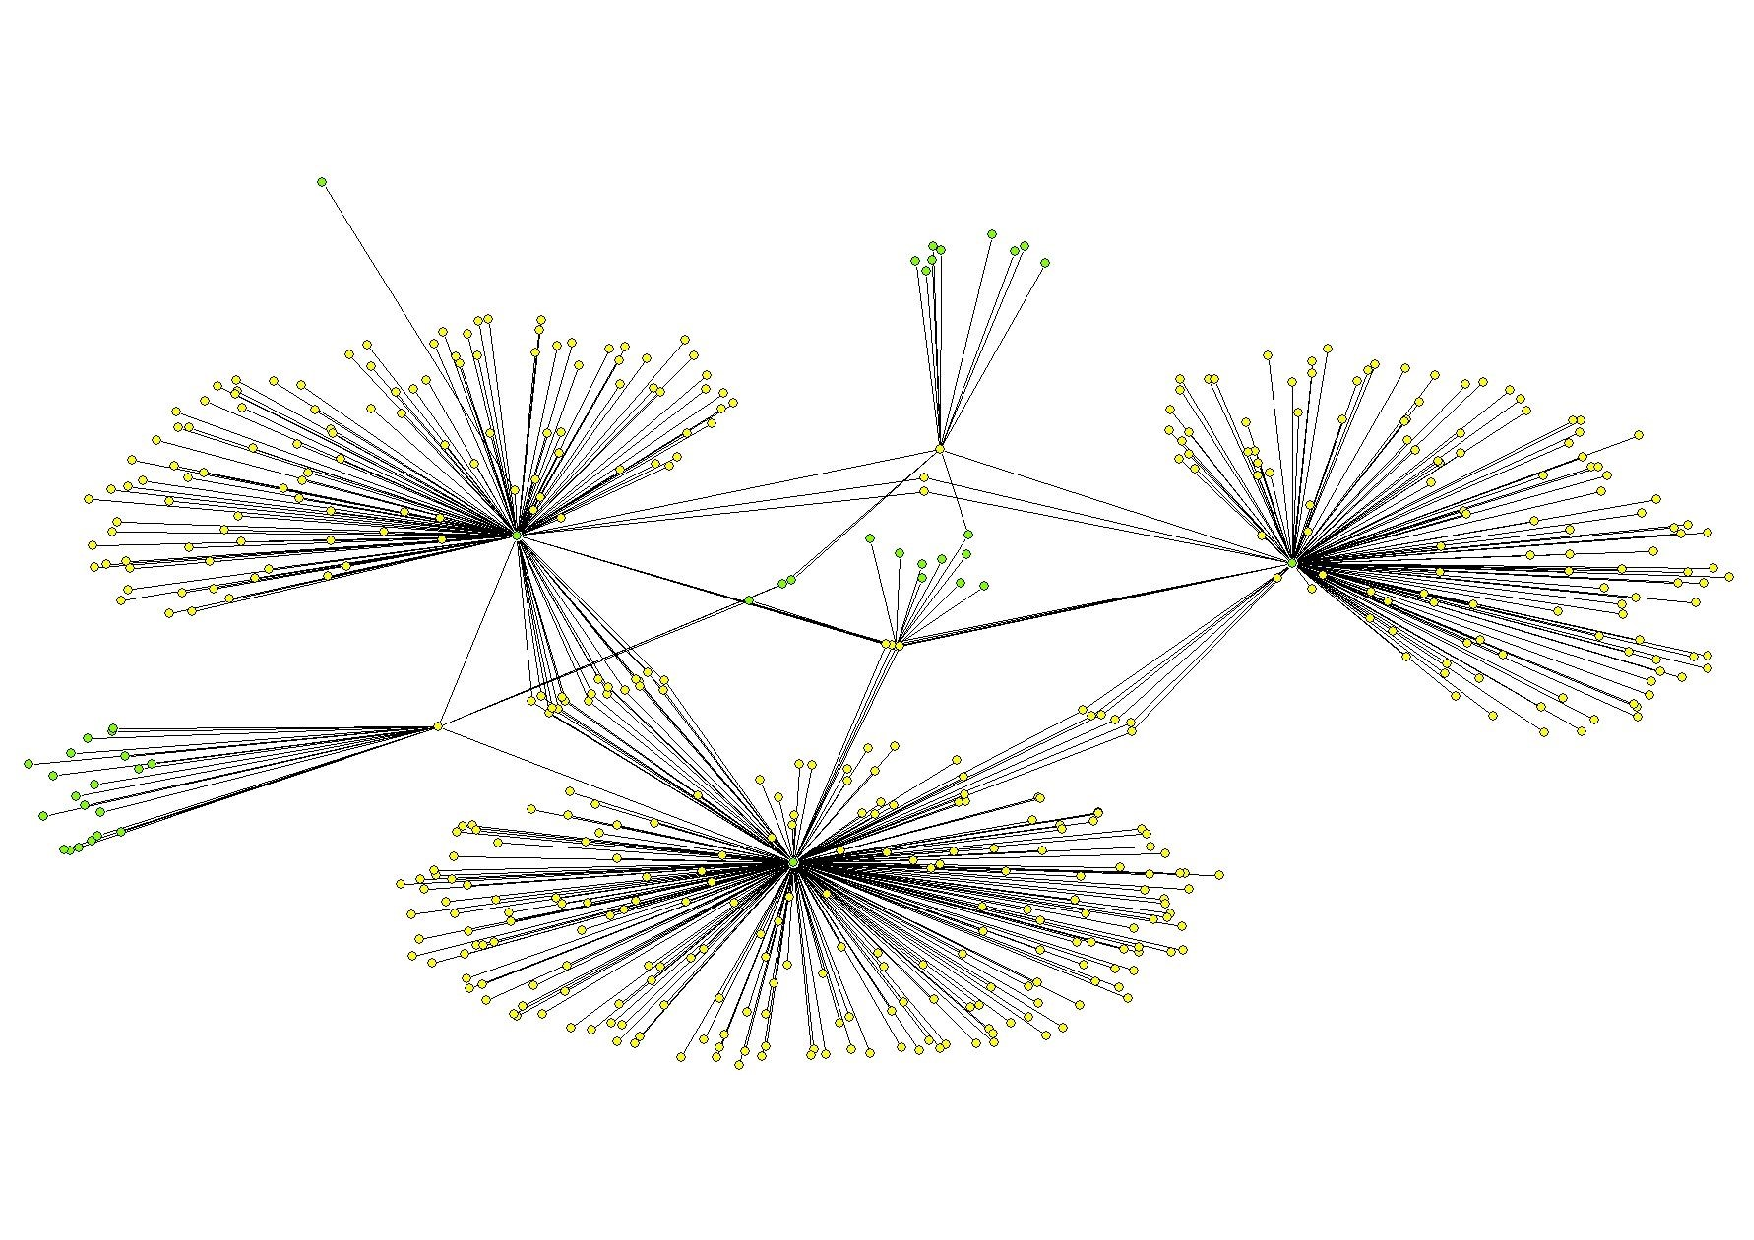
\includegraphics[scale=0.55]{rede_artistas_orquestras_PROVISORIO.pdf}
	\fonte{Elaboração do autor a partir de dados disponíveis online}
\end{figure}

Segundo \citeonline{denooy2011exploratory}, indivíduos podem construir laços diretamente entre si por onde fluem recursos, informação, status, etc. Por outro lado, a participação deles em eventos ou sua membresia em instituições ou organizações dá origem a um laço indireto entre indivíduos e entre instituições.

\begin{citacao}
	Na ciência política, economia e sociologia, muita atenção tem sido dada à composição de conselhos em grandes corporações. (\dots) Se uma pessoa é membro de um conselho de diretores em duas companhias, ele ou ela (\dots) é um diretor múltiplo que cria um diretorado conectivo ou uma conexão entre firmas. A rede de diretorados conectivos nos diz algo sobre a organização de um setor de negócios. É assumido que diretorados conectivos são canais de comunicação entre firmas\footnote{In political science, economy, and sociology, much attention has been paid to the composition of the boards of large corporations. (\dots) If a person is a member of the board of directors in two companies, he or she (\dots) is a multiple director who creates an interlocking directorate or interlock between firms. The network of interlocking directorates tells us something about the organization of a business sector. It is assumed that interlocking directorates are channels of communication between firms.}. \cite[p. 117]{denooy2011exploratory}
\end{citacao}

Do mesmo modo, os artistas convidados de uma orquestra são canais de comunicação entre elas onde fluem informação, métodos, técnicas e até mesmo prestígio. A partir dessa constatação, após o mapeamento de todas as instituições, usaremos os artistas como âncora para estabelecer uma rede de cooperação entre orquestras assumindo que o fluxo desses artistas é um indício das relações entre elas. Com a rede de cooperação, será possível identificar instituições que ocupam posições mais centrais e periféricas na estrutura social. Após uma combinação de medidas de centralidade e prestígio, buscaremos entender, através de uma investigação qualitativa, de que modo emerge das relações o \textit{standard} de qualidade com o qual todos assumem um compromisso tácito. 

%%%%%%%%%%%%%%%%%%%%%%%%%%%%%%%




\section{Cronograma de atividades}

Pretende-se que o início dos trabalhos na França junto ao prof. Lazega iniciem-se no final de outubro de 2017. Desse modo, a partir de 2017, no primeiro semestre o projeto final será submetido à banca de qualificação. De julho a setembro serão realizados os trabalhos em campo preliminares nas três capitais citadas, a saber, Belo Horizonte, Rio de Janeiro e São Paulo. No fim de outubro iniciaremos os trabalhos junto ao prof. Lazega que se estenderão por quatro meses. Após esse período, de volta ao Brasil, nos encarregaremos de complementar informações que se façam necessárias junto às orquestras pesquisadas enquanto nos ocupamos da redação do relatório da pesquisa (cf. Tabela \ref{cronograma}).

\begin{table}[!h]
\ibgetab{
\centering
\caption{Cronograma}
\label{cronograma}
}
{\begin{tabular}{rcp{5cm}}
	\hline
	\textbf{Atividade} & \textbf{Início} & \textbf{Tempo de realização} \\
	\hline
	Qualificação do projeto & Junho 2017 & O projeto está sendo desenvolvido desde fevereiro de 2016 \\
	\hline
	Pesquisa de campo & Julho 2017 & 3 meses \\
	\hline
	Viagem para Paris & Outubro 2017 & -- \\
	\hline
	Seminários ORIO & Novembro 2017 & 4 meses \\
	\hline
	Retorno ao Brasil & Fevereiro 2018 & -- \\
	\hline
	Relatório & Fevereiro 2018 & 12 meses \\
	\hline
	Pesquisa de campo & Junho 2018 & 3 meses \\
	\hline
	Defesa de tese & Fevereiro 2019 & -- \\
	\hline	
\end{tabular}
}
{}
\end{table}

\section{A contribuição deste trabalho para a promoção do ensino, formação e aprendizagem}

A Análise de Redes Sociais não configura meramente uma técnica de pesquisa ou um corpo teórico dentro de uma disciplina mas um paradigma a partir do qual o pesquisador vê o mundo. A realidade, na perspectiva das redes, é entendida como um produto das relações entre atores no mundo social. Este paradigma tem tomado grande força na ciência mundial em diversos campos do conhecimento (ciências da computação, biologia, neurociências, administração, economia, ciências sociais) e mais recentemente na academia brasileira.

No Brasil, este campo de estudos está em pleno desenvolvimento e poderá ser bastante fortalecido se acrescido dos últimos avanços conquistados em grande parte devido aos esforços do prof. Lazega. Seu grupo de pesquisa em Paris, ORIO (\textit{Observatoire des Réseaux Intra et Inter Organisationnel}) apresenta dois objetivos, um científico e outro prático\footnote{Informações disponíveis em \textless http://blogs.sciences-po.fr/recherche-network-organization-institution-dynamics-multilevel/recherche/\textgreater, acesso em 15/08/2016.}:

\begin{citacao}
O objetivo científico é melhorar nosso conhecimento de redes sociais e organizacionais para melhor compreender e modelizar o funcionamento de mecanismos sociais fundamentais da sociedade contemporânea, como as formas de aprendizagem, de solidariedade, de controle social, de regulação, etc., em particular à escala meso-social, intra e interorganizacional.

O objetivo prático é facilitar o acesso aos terrenos de pesquisa para doutorandos e pesquisadores confirmados, bem como ao financiamento de suas pesquisas. Em troca, nós trazemos à empresa, à instituição, à associação, uma capacidade de reconstituição, de visualização, de análise e de acompanhamento de suas redes socioeconômicas, intra e interorganizacionais.

Esta capacidade é hoje em dia indispensável para o \textit{Business Inteligence} e para o conhecimento do ambiente relacional complexo que abordamos dentro de uma perspectiva dinâmica e multinível\footnote{L’objectif scientifique est d’améliorer notre connaissance des réseaux sociaux et organisationnels pour mieux comprendre et modéliser le fonctionnement des mécanismes sociaux fondamentaux de la société contemporaine, tels que les formes d’apprentissage, de solidarité, de contrôle social, de régulation, etc., en particulier à l’échelle méso-sociale, intra- et inter-organisationnelle.\\
L’objectif pratique est de faciliter l’accès à des terrains de recherche pour doctorants et chercheurs académiques confirmés, ainsi qu’à des financements de ces recherches. En échange, nous apportons à l’entreprise, à l’institution, à l’association, une capacité de reconstitution, de visualisation, d’analyse et de suivi de ses réseaux socio-économiques, intra- et inter-organisationnels.\\
Cette capacité est aujourd’hui indispensable pour la veille stratégique et la connaissance de l’environnement relationnel complexe que nous abordons dans une perspective dynamique et multi-niveaux.}.
\end{citacao}

Esses objetivos vão ao encontro da proposta aqui apresentada na medida em que esta visa entender um complexo mercado brasileiro sob a perspectiva relacional. O conhecimento produzido junto ao ORIO será multiplicado no Brasil através das ações formativas empreendidas pelo GIARS\footnote{\url{www.giars.ufmg.br}} (Grupo Interdisciplinar de Pesquisa em Análise de Redes Sociais) do qual o autor faz parte. Essas ações formativas consistem de um \textit{workshop} anual específico sobre técnicas e métodos de ARS onde o autor também atua como professor e de seminários periódicos intitulados \textit{Seminários GIARS}.



\section{O potencial para o aumento da rede de pesquisa e educação, com novas técnicas e parcerias, além de ampla divulgação dos resultados}

O GIARS, grupo de pesquisa em ARS do qual o autor deste projeto faz parte, tem um trabalho significativo relacionado à divulgação e capacitação de alunos de graduação e pós-graduação, professores e pesquisadores para o uso das técnicas de ARS. A partir desse trabalho, uma rede com ramificações nacionais e internacionais se formou chegando até o ORIO, grupo de pesquisa coordenado pelo professor Lazega. A concretização deste estudo na França possibilitará a ampliação da rede de pesquisa brasileira através do contato com importantes pesquisadores parceiros do ORIO como Philippa Pattison, Julien Brailly, Eric Quintane e Tom Snijders.

Além disso, todos os resultados bem como os dados e códigos para análises e coleta de dados serão disponibilizados via \textit{github}\footnote{\url{https://github.com/}}, um repositório online aberto para compartilhamento de códigos de programação.

\section{A relevância para o desenvolvimento econômico e de bem estar social do Brasil no médio e longo prazos}

\subsection{O modelo de Baumol e Bowen -- a ``doença dos custos''}

William Baumol e William Bowen empreenderam, sob encomenda da Fundação Ford em 1965, uma pesquisa visando diagnosticar a situação econômica dos teatros da Broadway \cite{benhamou2007economia}. Seus achados são até hoje considerado válidos. Para \apudonline{baumol1966performing}{benhamou2007economia} a economia divide-se em dois setores, o setor 1 (arcaico) e o setor 2 (progressista). O setor arcaico não apresenta possibilidades de gerar ganhos de produtividade enquanto o setor progressista gera ganhos de produtividade a partir de inovações, de economias de escala e da acumulação de capital. A performance ao vivo faz parte do setor arcaico e isso se deve à posição que nele ocupa o trabalho. Para \citeonline{benhamou2007economia}

\begin{citacao}
	O trabalho é um elemento constitutivo do produto final: não se poderia substituí-lo sem desnaturar o produto. Não se poderia, por exemplo, substituir um dos instrumentistas de um quarteto de cordas por uma gravação\ldots Ora, os salários são iguais aos do setor progressista, devido à fluidez do mercado de trabalho; a consequência é um aumento permanente dos custos relativos do espetáculo ao vivo, que somente uma elevação dos preços das entradas pode compensar, com o risco de reduzir a demanda e as receitas. 
\end{citacao}

O modelo de \apudonline{baumol1966performing}{benhamou2007economia} baseia-se nas três hipóteses que se seguem:

\begin{enumerate}
	\item A economia divide-se em dois setores, arcaico e progressista. No setor arcaico, onde reside a performance ao vivo, a produtividade do trabalho é constante ou aumenta pouco e a quantidade de trabalho não pode ser diminuída sem desnaturar o produto. Sendo $L_{1,t}$ o volume de trabalho empregado no setor 1 no momento \textit{t} e \textit{a} um valor constante, a quantidade de produto no setor 1 no momento \textit{t} ($Y_{1,t}$) é obtida por $$Y_{1,t} = aL_{1,t}$$
	
	Sejam $Y_{2,t}$ e $L_{2,t}$ respectivamente a quantidade de produto do setor progressista no momento \textit{t} e o volume de trabalho empregado no setor 2 no momento \textit{t}, seja r a taxa de aumento da produtividade do trabalho e \textit{b} uma constante, a quantidade de produto no setor é obtido por $$Y_{2,t} = bL_{2,t}[1+r]^t $$
	
	\item Os custos de produção, comparados somente com os custos salariais (\textit{W}), evoluem no mesmo ritmo e sentido que a produtividade no setor progressista, isto é, $W_{1,t} = W_{2,t} = W_t = W[1+r]^t$. Os custos relativos de cada setor são, portanto, dados por
	$$C_1 = \frac{W_tL_{1,t}}{Y_{1,t}} = \frac{W(1+r)^tL_{1,t}}{aL_{1,t}} = \frac{W(1+r)^t}{a}$$
	$$C_2 = \frac{W_tL_{2,t}}{Y_{2,t}} = \frac{W(1+r)^tL_{2,t}}{bL_{2,t}(1+r)^t} = \frac{W}{b}$$
	
	Tem-se, então, que o custo por unidade de produto obtido aumenta indefinidamente no setor 1 e mantém-se constante no setor 2.
	
	\item ``A demanda de espetáculos ao vivo é elástica; toda alta de preço redunda numa redução do público'' \cite[p. 56]{benhamou2007economia}. Sendo os preços proporcionais aos custos relativos nos dois setores, $P_1 = \alpha C_1$ e $P_2 = \beta C_2$, então
	$$\frac{P_1Y_1}{P_2Y_2} = \frac{\alpha C_1Y_1}{\beta C_2Y_2} = Cte$$ ou
	$$\frac{C_1Y_1}{C_2Y_2} = \frac{W(1+r)^t \cdot L_{1,t}}{W(1+r)^t \cdot L_{2,t}} = \frac{L_{1,t}}{L_{2,t}} = K_0$$ e
	$$\frac{Y_1}{Y_2} = \frac{aL_{1,t}}{bL_{2,t}(1+r)^t} = \frac{aK_0}{b(1+r)^t}$$
	
	``Quando \textit{t} aumenta, $\frac{Y_1}{Y_2}$ diminui, e quando $t \rightarrow \infty$, $\frac{Y_1}{Y_2} \rightarrow 0$'' \cite[p. 57]{benhamou2007economia}. Desse modo, a produção do setor arcaico (1) diminui fatalmente.
\end{enumerate}

De forma complementar à lei de Baumol, \citeonline{throsby1994production} desenvolve uma função da produção do espetáculo ao vivo a qual pode ser sintetizada da seguinte forma:

O número de representações de uma determinada temporada deve ser fixado levando em conta a capacidade da sala \textit{v}. Sejam $L^s$ e $K^s$ o trabalho e o capital necessários para montar uma produção, sejam $L^r$ e $K^r$ o trabalho e o capital requeridos por cada representação da produção, o número de espectadores da iésima representação da jésima produção, $y_{ij}$, tal que $y_{ij} \leq v$, é dado por
$$y_j = \sum_iy_{ij} = y_i(L^{s}_{j}, K^{s}_{j}, m_j, q_j) $$ onde
o número de representações da jésima produção $$m_j = m_j(L^{r}_{j}, K^{r}_{j})$$ e $q_j$ resume as qualidades da jésima produção as quais, nesse contexto, podem ser medidas pela luxuosidade (\textit{lavishness}) da produção. Nesse caso, $q_j$ não é independente de $L^s$ e $K^s$. Espera-se que $$\frac{\partial y_j}{\partial m_j} > 0 \quad, \quad \frac{\partial^2y_j}{\partial m^{2}_{j}} < 0,$$ isto é, extender a temporada pode reduzir o número de espectadores na margem.

Segundo \citeonline[p. 59]{benhamou2007economia} ``a conclusão do modelo [de Baumol] é a inelutabilidade do aumento dos déficits dos espetáculos ao vivo''. Esse modelo tem sido corroborado por várias pesquisas \cite[e.g.]{throsby1979economics,leroy1980economie,peacock1983inflation,baumol1984inflation,dias2011artes} e, para \citeonline[p. 54]{benhamou2007economia}, essa característica do setor é suficiente para justificar o aumento das subvenções públicas e da prática do mecenato mesmo tendo em vista que ``essa intervenção maciça, distribuída de forma muito desigual, não é suficiente para garantir ao setor um equilíbrio financeiro duradouro''. Para \apudonline[p. 320]{baumol1966performing}{luksetich2011orchestras}, ``se se concorda que a artes de performance conferem benefícios gerais à comunidade como um todo\ldots as artes são bens públicos cujos benefícios demonstravelmente excedem as receitas que se espera coletar na bilheteria\footnote{If one agrees that the performing arts confer general benefits on the community as a whole\ldots the arts are public goods whose benefits demonstrably exceed the receipts one can hope to collect at the box office.}''.

A realização deste trabalho contribuirá não somente para o fortalecimento da política cultural no Brasil, mas também para um entendimento mais aprofundado sobre o funcionamento de seu mercado a partir da construção de conhecimento científico inédito acerca do objeto aqui proposto. Esse conhecimento será valioso na capacitação tanto de gestores culturais quanto gestores públicos.















\postextual
\citeoption{abnt-full-initials=yes}
\bibliography{BIBDOUTORADO, abnt-options}
\end{document}